%   Filename    : chapter_3.tex 
\chapter{Research Methodology}
\label{sec:methodology}

This chapter discusses the materials and methods to be employed in the study, focusing on the development requirements and the software, and languages utilized. This will also entail the overall workflow in conducting the study, Morphometric-Based Non-Invasive Sex Identification of Blood Cockles \textit{Tegillarca granosa} (Linnaeus, 1758) using machine learning technologies.

Dr. Victor Emmanuel Ferriols, the director of the Institute of Aquaculture, will oversee the overall workflow and conduct of this experiment. The researchers will also be guided by the research associates, LC Mae Gasit and Allena Esther Artera. Consequently, the whole dataset collection process will be done at the University of the Philippines Visayas hatchery facility. 

The methodology consists of seven parts: (1) Sample Collection, (2) Ethical Considerations, (3) Creating \textit{T.granosa} Dataset, (4) Morphological Characteristics Collection (5) Image Acquisition and Pre-processing, (6) Hardware and Software Configuration,(7) Morphometric Characteristics Evaluation Using Machine Learning


\section{Sample Collection}
\label{sec:samplecollect}
The collection of \Tgranosa samples used in this study is part of an ongoing research project by the UPV DOST-PCAARRD titled "Establishment of the Center for Mollusc Research and Development: Development of Spawning and Hatchery Techniques for the Blood Cockle (\textit{Anadara granosa}) for Sustainable Aquaculture." Furthermore, a total of 500 samples were provided in this study to classify the sex of \textit{T. granosa}.  The samples, ranging in size from 34 to 61 mm, are sourced from the coastal area of Zaraga, Iloilo, Philippines, and fish markets in Ivisan, Capiz, Philippines (\textit{see Figure~\ref{fig:granosa_shells}}). 

The research and experimentation take place at the University of the Philippines Visayas hatchery facility in Miagao, Iloilo, Philippines, where the samples are maintained in 200 L fiberglass reinforced plastic (FRP) tanks containing filtered seawater with 35 ppt salinity \cite{miranda2023}. 

As part of the data collection process, the researchers utilized induced spawning and dissection to classify the sex of the samples. Induced spawning through temperature fluctuations is the most natural and least invasive method for bivalves compared to other methods \cite{aji}. However, since not all samples exhibited gamete release, the researchers carried out a dissection process assisted by hatchery staff, to expedite data collection. The sex of the dissected samples is identified based on the coloration of gonad tissue, which varies by sex and maturity stage. Females exhibit orange-red to pale orange gonads while males display white to grayish-white gonads \cite{may2021}.  Provided that the methods used for data collection are noninvasive such that \textit{T. granosa} are oxygen regulators that are well adapted to tidal exposure to hypoxia \cite{davenport1986}

\begin{figure}[!htbp]
	\centering
	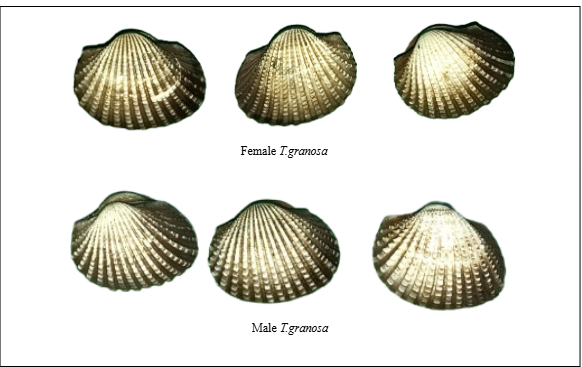
\includegraphics[width=0.9\textwidth]{figures/male-female T.granosa.png}
	\caption{Male and Female \Tegillarcagranosa shells}
	\label{fig:granosa_shells}
\end{figure}

\section{Ethical Considerations}
\label{sec:ethical}

The experiment involving blood cockles will be conducted according to the Animal Research: Reporting of In Vivo Experiments (ARRIVE) guidelines and will be reviewed by the Institutional Animal Care and Use Committee (IACUC) of the University of the Philippines Visayas. 

\section{Creating \textit{T. granosa} Dataset}
\label{sec:dataset}

The experiment began by collecting primary observations for 100 samples of \textit{T. granosa}. For the actual experimentation, the researchers will collect the original dataset by batch until a sample size of 500  \textit{T. granosa} is reached. Linear measurements were gathered by measuring the width, height, length, rib count, length of the hinge line, and distance between the umbos, and these measurements were organized in a CSV file. This dataset is essential for training and testing machine learning models and establishing the baseline for the Convolutional Neural Networks.

The images captured for each sample were saved in JPG format using a file naming convention that includes the sample sex, the orientation or view of the shell, and its corresponding number out of the total 500 samples. Female \textit{T. granosa} samples will have file names starting with 0, while males begin with 1. Each file name will include the views captured, such as (1) dorsal, (2) ventral, (3) anterior, (4) posterior, (5) left lateral, and (6) right lateral (refer to Figure~\ref{fig:granosa_views}), followed by a unique sample number. For example, “010001” will be the file name for the first female sample taken from the dorsal view, and “110001” will be the file name for the first male sample also taken from the dorsal view. This naming convention is designed to prevent data leakage and ensure that images are correctly labeled according to their respective samples. Assigning the naming convention ensures smooth flow in training and testing of the gathered data points. 

\begin{figure}[!htbp]
	\centering
	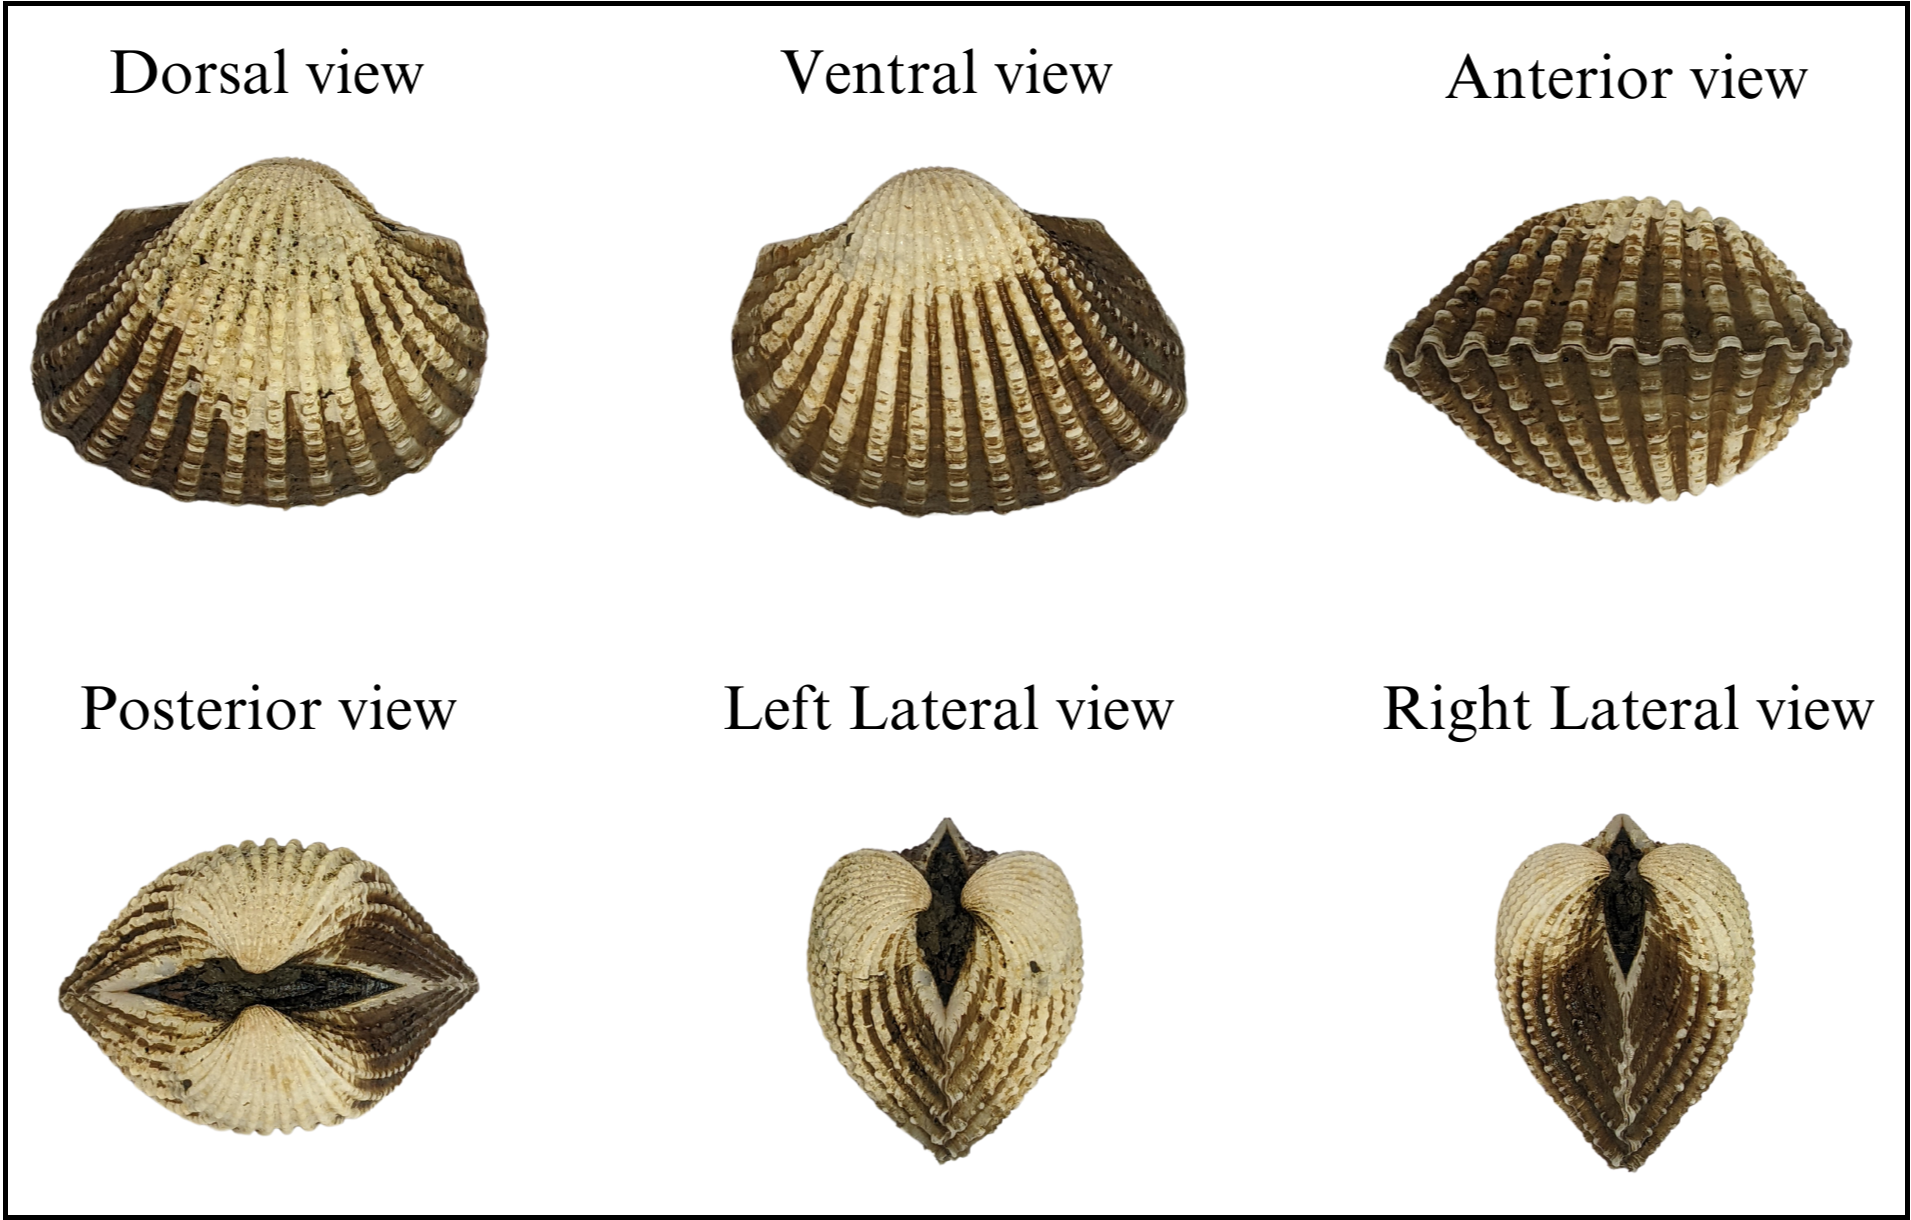
\includegraphics[width=0.9\textwidth]{figures/view.png}
	\caption{Different Views of the \textit{T. granosa} Shell Captured}
	\label{fig:granosa_views}
\end{figure}

\newpage
\section{Morphological and Morphometric Characteristics Collection}
\label{sec:morphochar}

Morphology refers to the biological form and represents one of the most visually recognizable phenotypes across all organisms \cite{tsutsumi2023}. In this study, morphological characteristics describe \textit{T. granosa} structural characteristics by measuring specific components, and dimensions such as shapes, sizes, and colors. In terms of morphometric characteristics, this refers to the measurable features of \textit{T. granosa} which are the length, width, height, length of the hinge line, the distance between the umbos, and the rib count. As stated by the researchers, quantifying and characterizing the shape is essential to understanding and visualizing the variations in \textit{T. granosa’s} morphology. 

In this study, the researchers measured the height, width, and length of \textit{T. granosa.} using a Vernier caliper to the nearest 0.01 mm. For the measurements, refer to Figure~\ref{fig:linear_measurements}. The length (A) of the \textit{T. granosa} refers to the measurement from the anterior to the posterior of the shell. The width (B) is the distance across the shell’s widest point from the left to the right valve. The height (C) refers to the measurement from the base of the shell to the shell’s apex. The length of the hinge line (D) near the hinge was measured, along with the distance between the umbos (E). 
Reyment and Kennedy (1998) indicated that incorporating rib count as supplementary information increases identification accuracy. Following this, the researchers recorded the rib count of the male and female \textit{T. granosa}, calculating the ratio since the sizes of the blood cockles vary. 

\begin{figure}[!htbp]
	\centering
	\includegraphics[width=0.95\textwidth]{figures/Tegillarca_granosa_linear_measurements.png}
	\caption{Linear Measurements of  \Tegillarcagranosa shell.}
	\label{fig:linear_measurements}
\end{figure}

\section{Image Acquisition and Data Gathering}
\label{sec:imageprocess}
This study will comprise 250 male and 250 female T. granosa images, resulting in a total of 3000 images taken from different angles. The researchers constructed a box-like structure with a white background to control the environment while capturing images of the samples. This setup aimed to maintain uniform captures of the images, fixing the camera at a consistent angle above the \textit{T. granosa}. A ring light was positioned in front of the box to ensure the image quality, eliminate shadows, and ensure the clarity of the sample during the image acquisition process. Google Pixel 3 XL is the smartphone used with the following specifications: 2960 x 1440 for the resolution, 4,032 x 3,024 pixels (12.2 MP) for the dimensions, f/1.8 for the fstop, 28mm (wide), ½.55”, 1.4µm, dual pixel PDAF, OIS \cite{concepcion2023}

\begin{figure}[!htbp]
	\centering
	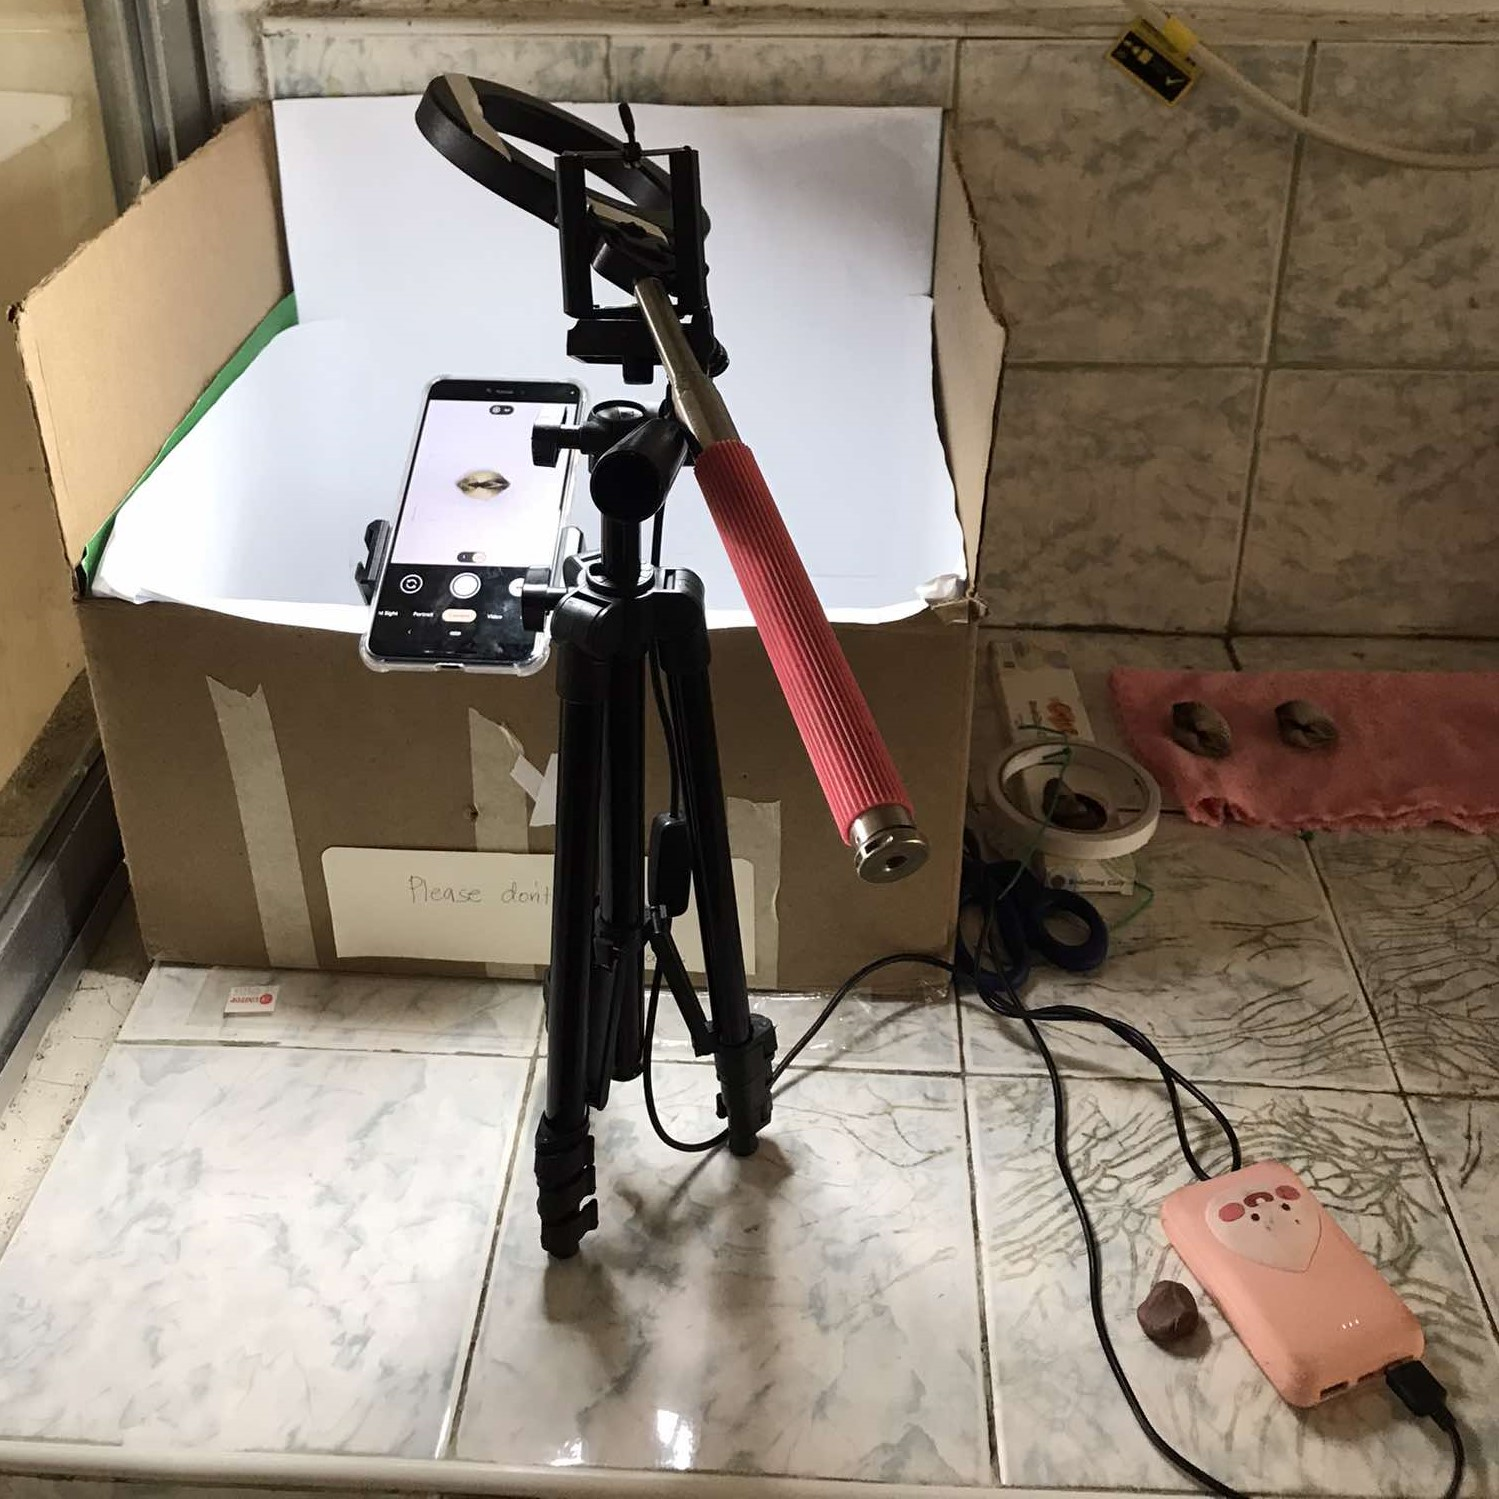
\includegraphics[width=0.4\textwidth]{figures/setup.jpg}
	\caption{Image Acquisition Setup for \textit{T. granosa} Samples}
	\label{fig: setup}
\end{figure}

\section{Hardware and Software Configuration}
This section of the paper discusses the software, programming language, and necessary tools for sex identification. Data collection, preprocessing, and model training were conducted on the Windows 11 operating system using an ACER Aspire 3 general-purpose unit (GPU) with an AMD Ryzen 3 7320U CPU with Radeon Graphics (8) @ 2.395 GHz and 8 gigabytes (GB) of memory. Google Collaboratory was utilized for collaborative preprocessing and data visualization. The results of the gathered measurements were stored and managed in a spreadsheet. GitHub was used for version control, documentation, and activity tracking throughout the study. Python served as the primary programming language, while MATLAB was used for machine learning operations and training machine learning algorithms.


\section{Morphometric Characteristics Evaluation Using Machine Learning }
\label{sec:ml models}

This section of the paper discusses the machine learning operations that serve as a baseline before delving into more complex deep learning methods for image classification. The study variables collected included linear measurements (length, width, height, length of the hinge line, distance between umbos, and rib count), along with additional features such as the length-width ratio and the length-height ratio as predictors. Samples were then classified by sex (female = 0, male = 1), which serves as the response variable.

\subsection{Preprocessing and Model Training}
\label{sec:pre-processing}

\begin{figure}[!htbp]
	\centering
	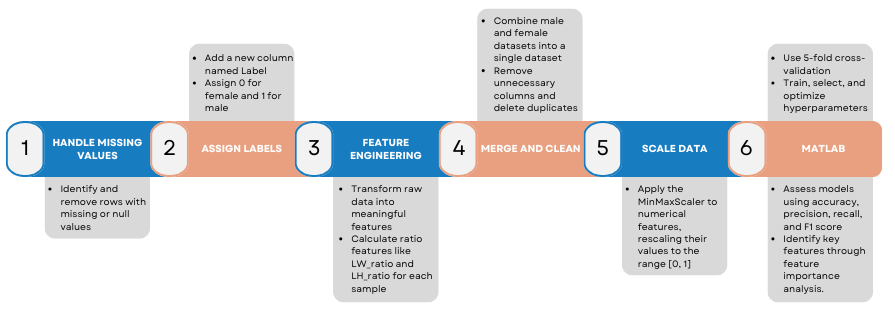
\includegraphics[width=0.8\textwidth]{figures/pipeline.png}
	\caption{Preprocessing and Model Training Pipeline}
	\label{fig: pipeline}
\end{figure}

The preprocessing of the dataset involved several steps as preparation for the machine learning analysis (\textit{see Figure~\ref{fig: pipeline}}). These steps included handling missing values, assigning labels, feature engineering, data merging and cleaning, and scaling the data. Missing values present in both male and female datasets were addressed by removing entries with NaN values. This approach ensured that subsequent analyses were performed on complete data, minimizing the risk of bias or errors and enhancing the reliability of the results.

Label assignment was conducted by creating a new column named "Label" in both datasets. A label of 0 was assigned to female samples, and a label of 1 was assigned to male samples, thereby establishing the target variable for the machine learning models.

In this study, the researchers performed feature engineering, which involves selecting, extracting, and transforming raw data into meaningful features suitable for accurate classification. Additional ratio-based features were introduced: Length-to-Width (LW\_ratio) and Length-to-Height (LH\_ratio), calculated separately for both male and female datasets. These features aimed to capture size-normalized morphometric traits to improve model performance and serve as a foundation for developing a more complex model for morphological classification using deep learning technologies.

Subsequently, the male and female datasets were merged to create a combined dataset for further machine learning analysis and exploration. Several operations were carried out to eliminate redundancy and potential bias by removing unnecessary columns and excluding duplicate rows to avoid bias in the analysis.

Lastly, numerical features were scaled using MinMaxScaler, which shifts and rescales the values to fit within a specific range, usually [0,1]. Scaling features uniformly helps machine learning models perform well, particularly for those sensitive to the varying scales of different features.

Moreover, machine learning operations, including model training and selection, were conducted using MATLAB Software version 24.2.0.2712019 (R2024b). A 5-fold cross-validation technique was applied to partition the dataset and assess accuracy in each fold. In MATLAB, researchers performed data standardization and model evaluation using metrics such as accuracy, precision, recall, and F1 score. Additionally, they determined the optimal hyperparameters and feature importance to identify the most relevant features for determining the sex of \textit{T. granosa}.



\subsection{Evaluation Metrics for Machine Learning}
Evaluating the performance of the binary classification model is important as well as selecting the appropriate metrics that is based on the requirements of the user. The performance of the supervised machine learning models will be measured based on four metrics namely: accuracy, precision, recall, and F1 score. 

Accuracy (ACC) is the ratio of the overall correctly predicted samples to the total number of examples in the evaluation dataset \cite{cui2020}. The overall correctness of the model in predicting male and female blood cockles. This metric could help in understanding how well the model performs across all classifications. The formula for the accuracy is: 

\begin{equation}
	\text{ACC} = \frac{\text{Correctly classified samples}} {\text{All samples }} = \frac{TP+ TN}{TP + FP + TN + FN}
	\label{eq:acc}
\end{equation}
Precision (PREC) is the ratio between correctly predicted samples in all samples that are assigned to the positive class \cite{cui2020}. This metric promotes fair representation and prevents the misidentification of blood cockles as it identifies potential inaccuracies or biases. The formula for precision is:


\begin{equation}
	\text{PREC} = \frac{\text{True positive samples}} {\text{Samples assigned to class }} = \frac{TP}{TP + FP}
	\label{eq:prec}
\end{equation}

Recall (REC) is known as the sensitivity or the true positive rate (TPR) which is the ratio of the correctly predicted cases from all the samples assigned to the actual positive cases \cite{cui2020}. This metric is the ability of the model to correctly identify positive male and female samples. The formula for the recall is:

\begin{equation}
	\text{REC} = \frac{\text{True positive samples}} {\text{Samples classified positive}} = \frac{TP}{TP + FN}
	\label{eq:rec}
\end{equation}

F1 score is defined as the mean of the precision and recall in which it penalizes the extreme values of either of the two \cite{cui2020}. The formula for the F1 is: 

\begin{equation}
	\text{F1} = \frac{ precision \times recall }{precision \times recall }= \frac{2 \times TP}{2 \times TP + FP + FN}
	\label{eq:f1}
\end{equation}




